\documentclass[12pt,a4paper]{article}

% Кодування/мови — в такому порядку
\usepackage[utf8]{inputenc}
\usepackage[T2A]{fontenc}
\usepackage[ukrainian]{babel}
\usepackage{cmap}            % коректний копіпаст з PDF (текстовий шар)
% (бажано мати шрифти cm-super у дистрибутиві)

\usepackage{geometry}
\geometry{left=2cm,right=2cm,top=2cm,bottom=2cm}

\usepackage{graphicx}
\usepackage{array,multirow,booktabs,makecell}
\usepackage{caption}
\renewcommand{\thetable}{\arabic{table}}
\usepackage[table]{xcolor} % <-- це дає \rowcolor і \cellcolor
\captionsetup[table]{name=Таблиця}

\usepackage{amsmath}
\usepackage{pdflscape}
\usepackage{xcolor}

% Гіперпосилання — тримай наприкінці пакетів, з unicode
\usepackage[unicode]{hyperref}

\begin{document}

    \begin{titlepage}

        % Картинка шапки (по центру, з відступом від верху)
        \begin{center}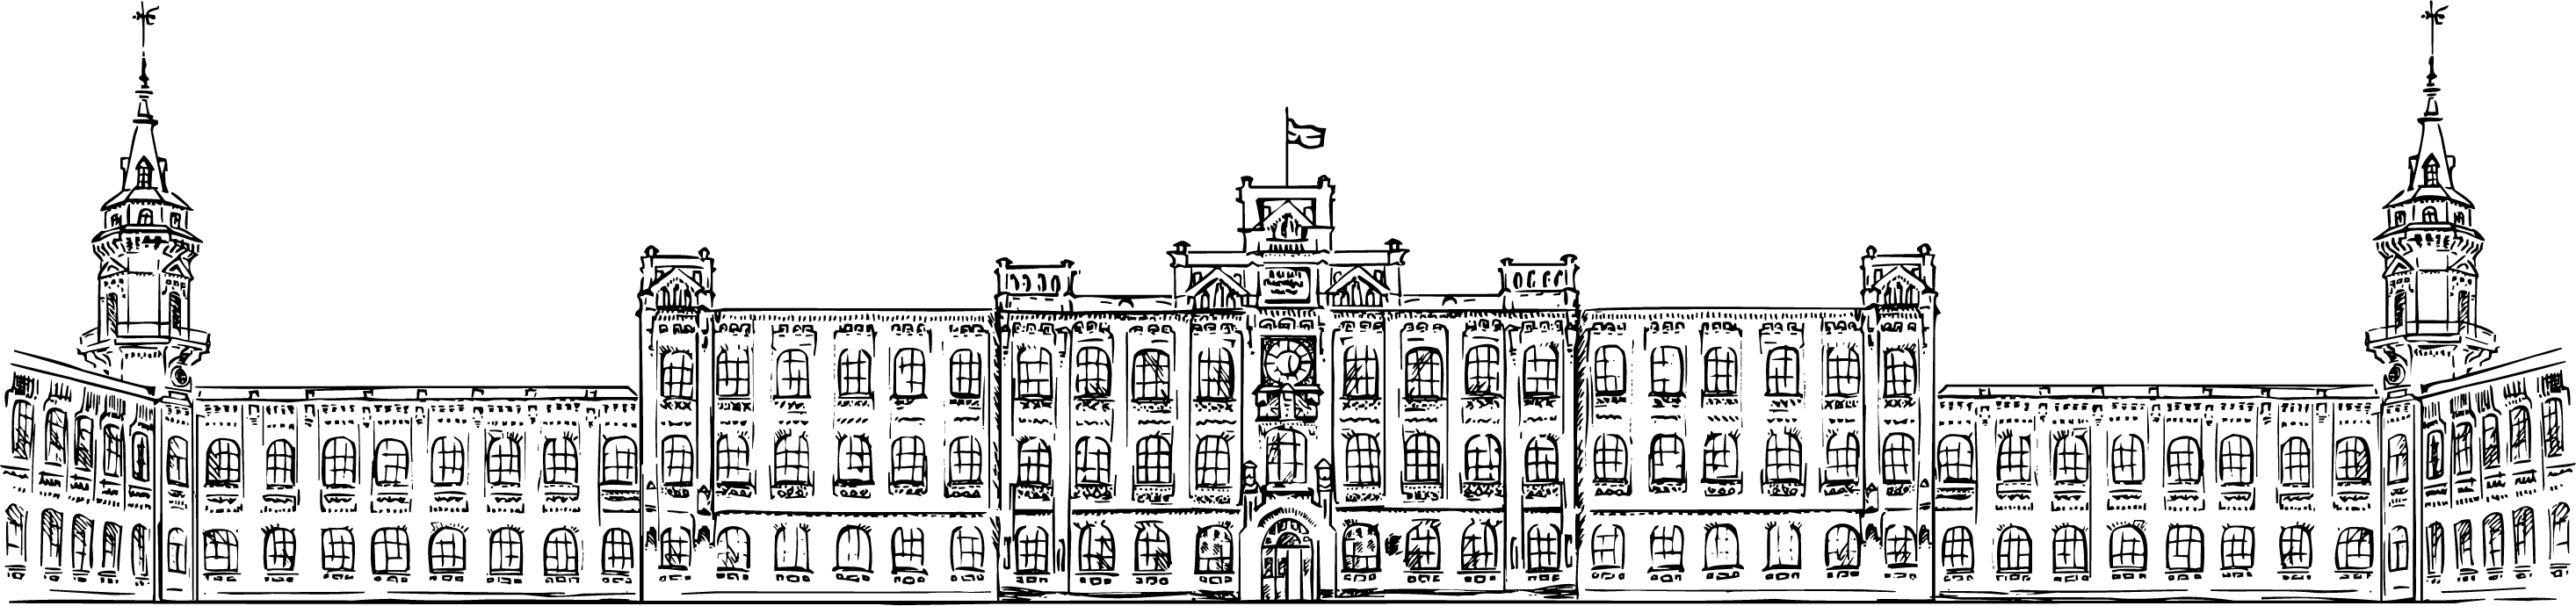
\includegraphics[width=0.7\textwidth]{../../../TITLES/letterhead.png}\end{center}

        \begin{center}
            \large Національний технічний університет України\\
            «Київський політехнічний інститут імені Ігоря Сікорського»\\[1em]
            Факультет інформатики та обчислювальної техніки\\
            Кафедра обчислювальної техніки
        \end{center}

        \vfill

        \begin{center}
            \textbf{\LARGE Теорія електричних кіл та сигналів}\\[2em]
            \textbf{\Large Лабораторна робота №3}\\
            «Використання системи комп’ютерної алгебри для розрахунку однофазного електричного кола»
        \end{center}

        \vfill

        \begin{flushright}
            Виконав: студент 2 курсу ФІОТ, гр. ІО-41\\
            \textit{Давидчук А.~М.}\\[1em]
            Перевірив: \textit{Лободзинський В.~Ю.}
        \end{flushright}

        \vfill

        \begin{center}Київ --- 2025\end{center}

    \end{titlepage}

    \setlength{\parindent}{0pt}

    \textbf{\underline{Тема:}} «Використання системи комп’ютерної алгебри для розрахунку однофазного електричного кола».

    \vspace{1em}

    \textbf{\underline{Мета:}} Навчитися використанням системи комп’ютерної алгебри для розрахунку однофазного електричного кола змінного струму.

    \begin{center} \textbf{\large Практична частина} \end{center}

    \setlength{\parindent}{1.5em}

    Усі розрахунки було проведено за допомогою мови програмування Python (вихідний код додано разом із звітом)

    Моя група: ІО-41, мій порядковий номер у групі: 6. Звідси $N = 6$, $S = 1$.
    Звідси загальна структурна схема електричного кола:
    \begin{figure}[h!]

        \renewcommand{\thefigure}{\arabic{figure}} % робимо "3.1", "3.2" і т.д.

        \centering
        % Підставляєте потрібний шлях та розмір зображення:
        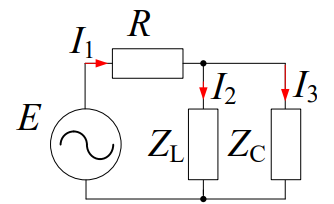
\includegraphics[width=0.3\textwidth]{scheme0.png}
        % Підпис (зазвичай під малюнком):
        \caption{Структурна схема електричного кола}
        % Мітка для посилань у тексті (\ref{fig:...})
        \label{fig1:scheme0}

    \end{figure}

    А також приймаючи, що частота синуссинусоїдальної напруги $f = 50$ Гц.

    Відповідно до таблиці варіантів параметрів елементів електричного кола, при $N=6$ маємо:
    
    \begin{table}[h]
    \centering
    \begin{tabular}{|c|c|c|c|c|c|}
    \hline
    \textit{E}, В & \textit{R}, Ом & $Z_{L}$, Ом & $\varphi_{L}$, град & $Z_{C}$, Ом & $\varphi_{C}$, град \\
    \hline
    \rule{0pt}{12pt} 17 & 220 & 142 & 42 & 240 & -83\\  % порожній рядок
    \hline
    \rowcolor[HTML]{D9D9D9}
    -- & -- &
    \cellcolor{white}\makecell[l]{$R_{L}=105{,}506$\\$X_{L}=94{,}998$} &
    -- &
    \cellcolor{white}\makecell[l]{$R_{C}=29{,}28$\\$X_{C}=-238{,}32$} &
    -- \\
    \hline
    \end{tabular}
    \caption{Параметри елементів однофазного електричного кола}
    \end{table}

    Оскільки в задачі не вказано про початкову фазу ЕРС, то вважатимемо її рівною нулю: $\varphi_0 = 0$ град. Звідси
    ЕРС можна записати як: $E = 17 e^{j0\text{\textdegree}} = 17 + 0j$ В.

    На основі структурної схеми електричного кола побудовано схему заміщення шляхом заміни імпедансів еквівалентними ідеалізованими елементами:

    \begin{figure}[h!]

        \renewcommand{\thefigure}{\arabic{figure}} % робимо "3.1", "3.2" і т.д.

        \centering
        % Підставляєте потрібний шлях та розмір зображення:
        \includegraphics[width=0.3\textwidth]{scheme1.pdf}
        % Підпис (зазвичай під малюнком):
        \caption{Схема заміщення однофазного електричного кола}
        % Мітка для посилань у тексті (\ref{fig:...})
        \label{fig1:schema}

    \end{figure}

    Тепер будемо проводити обчислювання струмів $I_1$, $I_2$ та $I_3$. Спершу запишемо імпенданси кожного елемента кола в комплексній формі (приймаючи $j = \sqrt{-1}$):

    \[
    \vec{Z} = 
    \begin{pmatrix}
    Z_1 = 220 \\
    Z_2 = 105{,}506 + j 94{,}998 \\
    Z_3 = 29{,}28 - j 238{,}32
    \end{pmatrix}
    \]

    На основі схеми запишемо рівняння за першим і другим законами Кірхгофа та розв'яжемо СЛАР:

    \[
    \left\{
    \begin{aligned}
    I_1 Z_1 + I_2 Z_2 - E &= 0,\\
    I_1 Z_1 + I_3 Z_3 - E &= 0,\\
    I_1 - I_2 - I_3 &= 0.
    \end{aligned}
    \right.
    \]

    Звідси отримаємо:
    
    \[I_1 = 0{,}043 + -0{,}002j = 0{,}043 e^{-j2.538\text{\textdegree}}\]
    \[I_2 = 0{,}041 - 0{,}033j = 0{,}053 e^{-j38.776\text{\textdegree}}\]
    \[I_3 = 0{,}002 + 0{,}031j = 0{,}031 e^{j86.22\text{\textdegree}}\]

    І зведемо ці значення у таблицю:

    \begin{table}[h]
    \centering
    \renewcommand{\arraystretch}{1.35}
    \begin{tabular}{|c|c|c|c|}
    \hline
    \multirow{2}{*}{} & $I_1$, А & $I_2$, А & $I_3$, А \\
    \cline{2-4}
    \hline
    алгебраїчна форма
    & $\displaystyle 0{,}043 + -0{,}002j$
    & $\displaystyle 0{,}041 - 0{,}033j$
    & $\displaystyle 0{,}002 + 0{,}031j$ \\
    \hline
    показникова форма
    & $\displaystyle 0{,}043 e^{-j2.538\text{\textdegree}}$
    & $\displaystyle 0{,}053 e^{-j38.776\text{\textdegree}}$
    & $\displaystyle 0{,}031 e^{j86.22\text{\textdegree}}$ \\
    \hline
    \end{tabular}
    \caption{\centering Обчислені комплексні значення струмів у алгебраїчному та показниковому формах}
    \end{table}

    Тепер перевіримо правилність обчислення струмів за допомогою методу балансу потужностей:

    Нехай потужність усіх джерел ЕРС дорівнює $S_E = \sum_k S_{E_k}$, а всіх споживачів $S_D = \sum_m S_{D_m}$, тоді:

    \[
    S_E = S_D \Rightarrow \sum_k S_{E_k} = \sum_m S_k \text{Вт}
    \]

    де $S_{E_k} = E_k \cdot I_k$, а $S_k = U_k \cdot I_k = I^2_k / Z_k$.

    У нашому випадку маємо:

    \[
    S_E = E \cdot I_1
    \]
    \[
    S_D = I_1^2 Z_1 + I_2^2 Z_2 + I_3^2 Z_3
    \]

    Обчисливши за допомогою Python отримаємо такі значення:

    \[
    S_E = 0{,}735 - 0{,}033j = 0{,}736 e^{-j2.538^\circ} \text{ Вт}
    \]
    \[
    S_D = 0{,}735 - 0{,}033j = 0{,}736 e^{-j2.538^\circ} \text{ Вт}
    \]

    Звідси висновуємо, що баланс потужностей виконується, отже обчислення струмів вірні.

    Також окремо можна виділити активну $P$, реактивну потужності $Q$ джерел та повну комплексну потужність джерела $S$:

    \[
    P = \Re (S_D) = 0{,}735 \text{Вт}, \quad Q = \Im (S_D) = -0{,}033 \text{ Вт}, \quad S = \left| S_E \right| = 0{,}736 \text{ Вт}
    \]

    Зведемо всі обчислені значення потужностей до однієї таблиці:

    \newcommand{\g}{\cellcolor[gray]{0.85}} % сірий фон клітинки

    \begin{table}[h]
    \renewcommand{\arraystretch}{1.35}
    \setlength{\tabcolsep}{8pt}
    \centering
    \begin{tabular}{|>{\raggedright\arraybackslash}p{7.8cm}|c|c|c|}
    \hline
    & $S$, Вт & $P$, Вт & $Q$, Вар \\
    \cline{2-4}
    \hline
    повна комплексна потужність джерела
    & 0{,}736 & 0{,}735 & -0{,}033 \\
    \hline
    активна потужність споживачів
    &  \g-- & 0{,}735 & \g-- \\
    \hline
    реактивна потужність споживачів
    &  \g-- & \g-- & -0{,}033 \\
    \hline
    \end{tabular}
    \caption{Обчислені абсолютні значення потужностей}
    \end{table}
    
    Залишилося розрахувати комплексні значення напруг у колі:

    \[
    \vec{U} = 
    \begin{pmatrix}
    U_R = I_1 \cdot R \\
    U_{R_L} = I_2 \cdot R_L \\
    U_L = I_2 \cdot j \cdot X_L \\
    U_{R_C} = I_3 \cdot R_C \\
    U_C = I_3 \cdot (-j \cdot X_C) 
    \end{pmatrix} =
    \begin{pmatrix}
    9{,}513 -0{,}422j = 9{,}522 e^{-j2{,}538^\circ} \\
    4{,}345 -3{,}49j = 5{,}573 e^{-j38{,}776^\circ} \\
    3{,}143 + 3{,}912j = 5{,}018 e^{j51{,}224^\circ} \\
    0{,}06 + 0{,}912j = 0{,}914 e^{j86{,}22^\circ} \\
    -7{,}427 + 0{,}491j = 7{,}443 e^{j176{,}22^\circ}
    \end{pmatrix}
    \]

    І для зручності зведемо обчислені значення до однієї таблиці:

    \begin{table}[h]
    \centering
    \renewcommand{\arraystretch}{1.35}
    \begin{tabular}{|c|c|c|c|c|c|}
    \hline
    & $U_{R}$, В & $U_{R_L}$, В & $U_{L}$, В & $U_{R_C}$, В & $U_{C}$, В \\
    \cline{2-6}
    \hline
    алг. форма
    & $\displaystyle 9{,}513 -0{,}422j$
    & $\displaystyle 4{,}345 -3{,}49j$
    & $\displaystyle 3{,}143 + 3{,}912j$
    & $\displaystyle 0{,}06 + 0{,}912j$
    & $\displaystyle -7{,}427 + 0{,}491j$\\
    \hline
    пок. форма
    & $\displaystyle 9{,}522 e^{-j2{,}538^\circ}$
    & $\displaystyle 5{,}573 e^{-j38{,}776^\circ}$
    & $\displaystyle 5{,}018 e^{j51{,}224^\circ}$
    & $\displaystyle 0{,}914 e^{j86{,}22^\circ}$
    & $\displaystyle 7{,}443 e^{j176{,}22^\circ}$ \\
    \hline
    \end{tabular}
    \caption{Обчисленні комплексні значення напруг в алгебраїчній та показниковій формах}
    \end{table}

    Також окремо, я обчислив значення циклічної частоти $\omega$, значення індуктивності котушки та ємності конденсатора:

    \[
    \omega = 2\pi f = 100 \pi \quad
    \]
    \[
    X_L = \omega L \Rightarrow L = \frac{X_L}{\omega} \approx 0{,}302 \text{ Гн} \quad
    \]
    \[
    X_C = -\frac{1}{\omega C} \Rightarrow C = -\frac{1}{\omega X_C} \approx 13{,}356 \text{ мкФ}
    \]

    На основі всіх обчислених значень побудую електричну схему в програмі Multisim:

    \begin{figure}[h!]

        \renewcommand{\thefigure}{\arabic{figure}} % робимо "3.1", "3.2" і т.д.

        \centering
        % Підставляєте потрібний шлях та розмір зображення:
        \includegraphics[width=0.5\textwidth]{scheme2.pdf}
        % Підпис (зазвичай під малюнком):
        \caption{Однофазна електрична схема в програмі Multisim}
        % Мітка для посилань у тексті (\ref{fig:...})

    \end{figure}

    \newpage

    Побудова векторної діаграми струмів та напруг:

    \begin{figure}[h!]

        \renewcommand{\thefigure}{\arabic{figure}} % робимо "3.1", "3.2" і т.д.

        \centering
        % Підставляєте потрібний шлях та розмір зображення:
        \includegraphics[width=1.0\textwidth]{Figure_1.pdf}
        % Підпис (зазвичай під малюнком):
        \caption{Векторні діаграми комлпексних напруг та струмів}
        % Мітка для посилань у тексті (\ref{fig:...})

    \end{figure}

    З неї видно, що всі обчислення провелись успішно (сума напруг дорівнює $=E$, і сума струмів $=I_1$)

    \vspace{1em}

    \setlength{\parindent}{0em}

    \textbf{Висновок:} У роботі продемонстровано застосування фазорного підходу та комплексних імпедансів для аналізу однофазного кола змінного струму. На основі схеми заміщення складено та розв’язано систему лінійних рівнянь для струмів у гілках, після чого обчислено комплексні напруги на елементах у алгебраїчній та показниковій формах. Коректність розрахунків підтверджено енергетично та топологічно: виконано баланс потужностей (сума потужностей споживачів дорівнює комплексній потужності джерела), а також перевірено закони Кірхгофа на векторних діаграмах (суми напруг по контурах збігаються з ЕРС; сума струмів у вузлі дорівнює струму джерела).

    \setlength{\parindent}{1.5em}

    Додатково з амплітудно-фазових параметрів імпедансів визначено еквівалентні значення $L$ та $C$, що забезпечило узгодження аналітичної моделі з моделюванням у середовищі Multisim. Отримані результати підтверджують правильність обраної методики та придатність Python/NumPy для відтворюваних інженерних розрахунків і побудови наочних векторних діаграм. 

\end{document}